 We used \ac{SynLBD} \cite{SynLBD20}  together with confidential 
\ac{BDS} microdata (as of June 2015) for \ac{BDS} tabulations 
by establishment age and size ({\tt bds\_e\_agesz}), creating  \textbf{BDS$^{(s)}$} 
and 
\textbf{BDS$^{conf}$}, respectively. For the published data \textbf{BDS$^{(0)}$}, we used data 
from the September 2014 release. 
%\margincomment{LV}{I added this note, since it's necessary to explain the discrepancy in the estabBirths statistic - there shouldn't be any difference if really using the same input data, since there are no suppressions, but identifier corrections lead to discrepancies in that particular statistic}
We note that the \ac{BDS} microdata is thus of more recent vintage, and contains some 
improvements in the underlying data. This leads to certain discrepancies in the results, as will be 
evidenced in the tables. 
Using Algorithm~1 and combining \textbf{BDS$^{(0)}$}  and \textbf{BDS$^{(s)}$}, we created 
\textbf{BDS$^{(i)}$} and 
\textbf{BDS$^{(in)}$}. Using Algorithm~2 and combining the microdata underlying 
\textbf{BDS$^{(s)}$} 
and 
\textbf{BDS$^{conf}$}, we created \textbf{BDS$^{(ii)}$} with $n=4$, linear $w_{js}$, and $p=0$. %
%
%\footnote{$w_{j\cdot} = \left \lbrace 0, 0.2, 0.4, 0.6, 0.8 \right \rbrace$ and $\tilde{w}_{jt} = 1 - 
%w_{jt}$. }
%
Further variation of the weights $w_{js}$ and of $n$ lead to \textbf{BDS$^{(ii)}(w=0) =$  
BDS$^{(iiw)}$}%
%\footnote{$w_{j\cdot} = \left \lbrace 0, 0, 0, 0, 0 \right \rbrace$ and $\tilde{w}_{jt} = 1 - w_{jt}$. }  
 and 
\textbf{BDS$^{(ii)}(n=0) =$ BDS$^{(iin)}$}, %
%\footnote{$w_{j\cdot} = \left \lbrace 0, 1, 1, 1, 1 \right \rbrace$ and $\tilde{w}_{jt} = 1 - w_{jt}$. }  
respectively. We create \textbf{BDS$^{(n)}$} with $c=10$ and $d=25$ percent the brackets of the noise distribution.


The analysis is restricted to 1977-1999 because \ac{SynLBD} version 2.0 is only available through 
2001, and we chose to avoid any issues at the boundaries of the data. %\margincomment{Lars}{Why did I choose 1999 and not 2001?}
%
As noted in Table~\ref{tab:bds_e}, about 26\% of all cells in publicly available 
\textbf{BDS$^{(0)}$} 
have some 
suppression. For this version of the paper, we analyzed two variables, ``Job Creation by 
establishment births'' ({\tt job\_creation\_births}) and ``Job Creation by 
continuing establishments'' ({\tt job\_creation\_continuers}). Other variables, such as the 
number of establishments ({\tt estabs}) and ``Employment'' ({\tt emp}), which are never 
suppressed, 
serve as a benchmark.

\subsection{Extent of protection}
\label{sec:protection}
\input{protection}
Protection of the table relies in large part on the fact that the data replacing the suppressions is 
itself synthetic, and released (in the case of the examples in this paper) or (potentially) 
releasable (for tabulations with geography) to a broad audience \cite{AbowdVilhuber2010}. No 
establishment's observed data is released in the SynLBD, and only the industry distribution of 
establishments is preserved exactly.%
%
\footnote{To be precise, the number of establishments that ever exist within each 3-digit 
\ac{SIC} throughout the timeframe of the synthesis is preserved exactly. At any given point of 
time, though, that number will diverge from the confidential number. }
%
 A detailed analysis, based in part on a comparison of the 
confidential and synthetic microdata is 
provided elsewhere \cite{KinneyEtAl2011}. Very few synthetic values are close to the 
corresponding confidential values, and \cite{KinneyEtAl2011} conclude that the synthetic 
microdata is not disclosive of the confidential microdata. It follows that tabulations of 
non-disclosive microdata are themselves not disclosive.

We do, however, note that one particular attribute present on the confidential microdata - 
geography - was not included on the released synthetic microdata. Several of the tabulations 
listed in Table~\ref{tab:bds_e} and~\ref{tab:bds_f} are cross-tabulated by geography. Two 
options thus arise: (i) to release a version of the SynLBD with protected geography (see 
ongoing work \cite{KinneyEtAl2013}), and then use that version for tabulations; (ii) to 
create a non-released version of the SynLBD that may not satisfy the criteria for release at the microdata level, but does allow for the computation of releasable tabulations. Neither of these options are explored in the present article.

\subsection{Aggregate differences}

The present version of the \ac{SynLBD}, created in 2011, has some small aggregate differences with the released 
\ac{BDS} tables. Our analysis will not take any particular measures to alleviate the bias. 
Figure~\ref{fig:level_denom} shows  aggregated \texttt{denom} (average employment), job 
creation, and job creation by establishment births and continuing establishments, and 
Figure~\ref{fig:pct_denom} presents the percentage difference between the released data and 
the synthetic data at the most aggregated level, for the same variables. We note that 
whereas total employment is only marginally lower in the synthetic data at any point in time, synthetic job creation is significantly higher. The 
synthetic data underestimates job creation by establishment births, and overestimates job 
creation by continuing establishments. These points were originally highlighted elsewhere 
\cite{KinneyEtAl2011}, and are being addressed in the next iteration of the \ac{SynLBD}.
%\margincomment{LV}{This could still use a comparison of the Algorithm 2 final output datasets}


%\begin{figure}
%	\centering
%	\caption{Levels of released and synthetic data\label{fig:level_denom}}
%	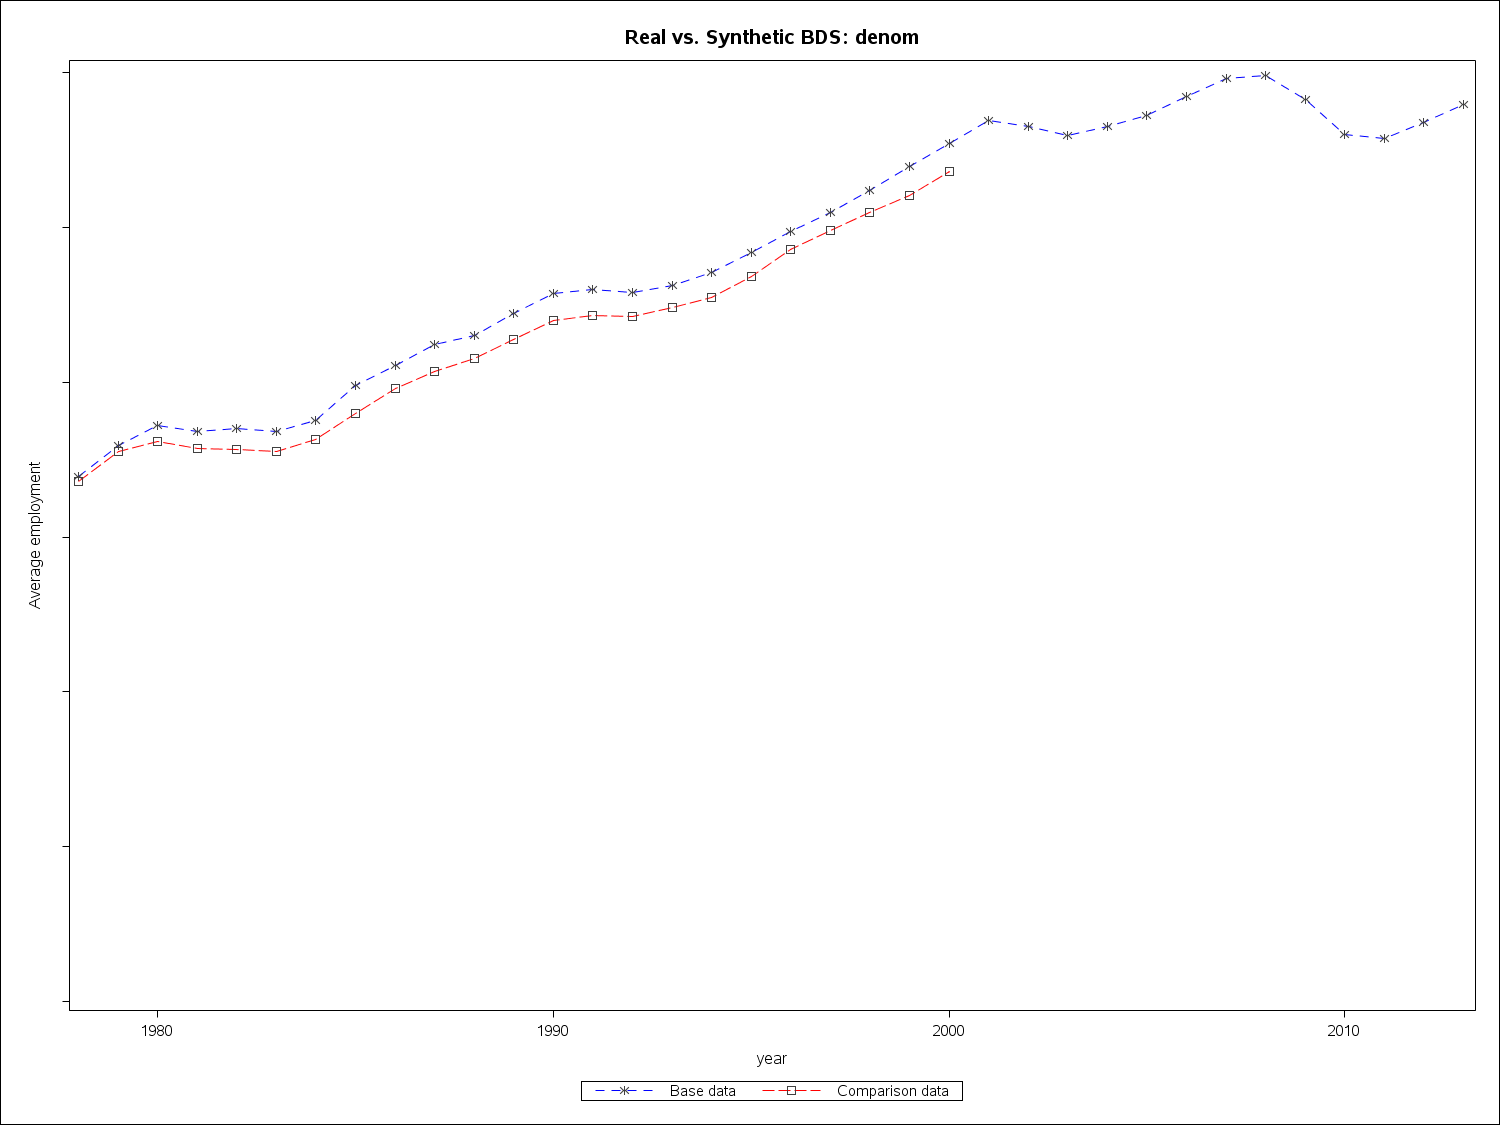
\includegraphics[width=0.45\textwidth]{results/graph_bds_real_vs_syn_denom}
%	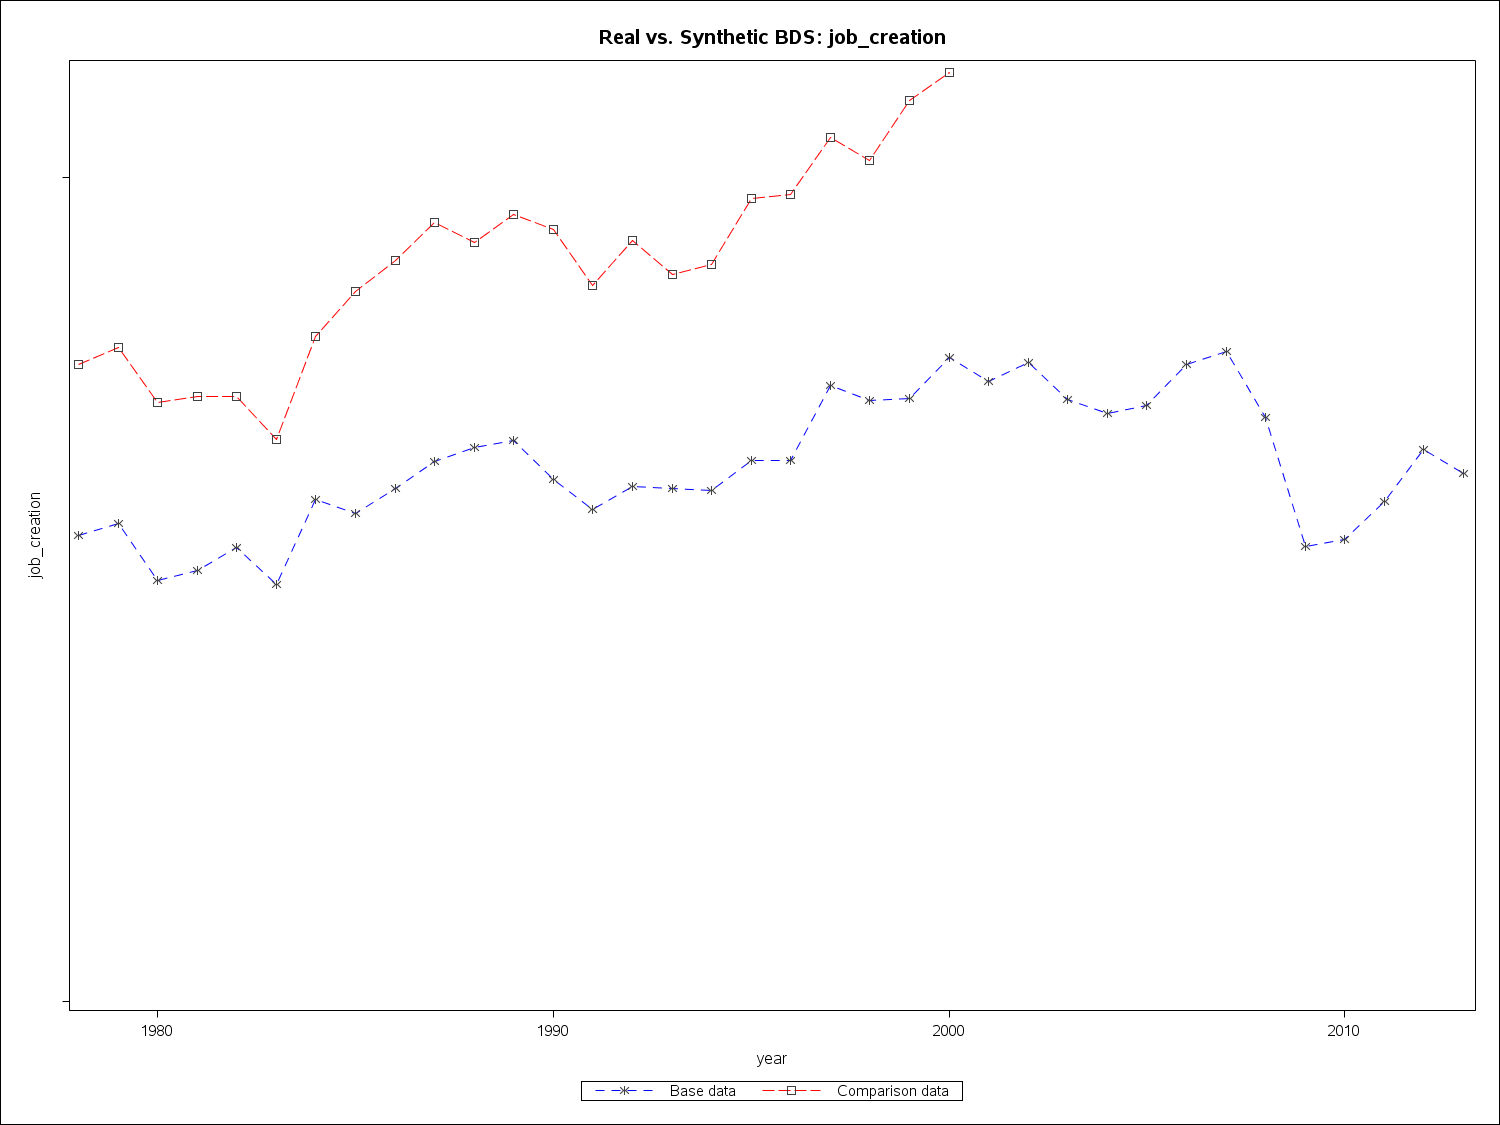
\includegraphics[width=0.45\textwidth]{results/graph_bds_real_vs_syn_job_creation}
%	
%	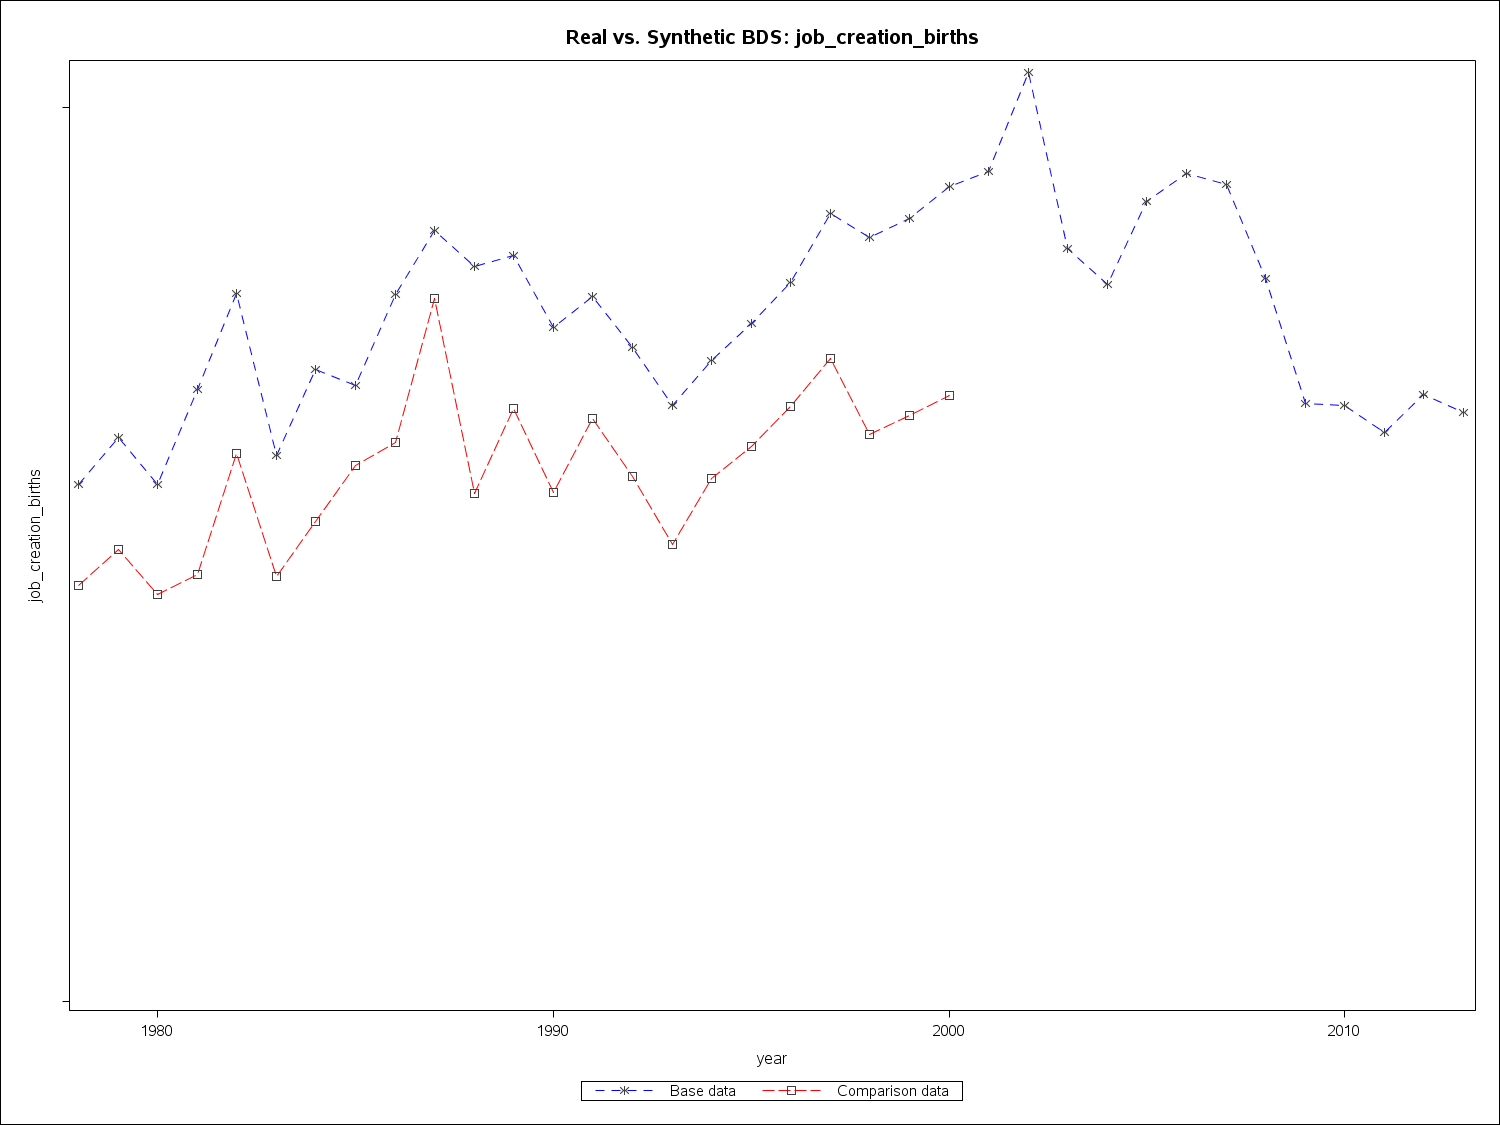
\includegraphics[width=0.45\textwidth]{results/graph_bds_real_vs_syn_job_creation_births}
%	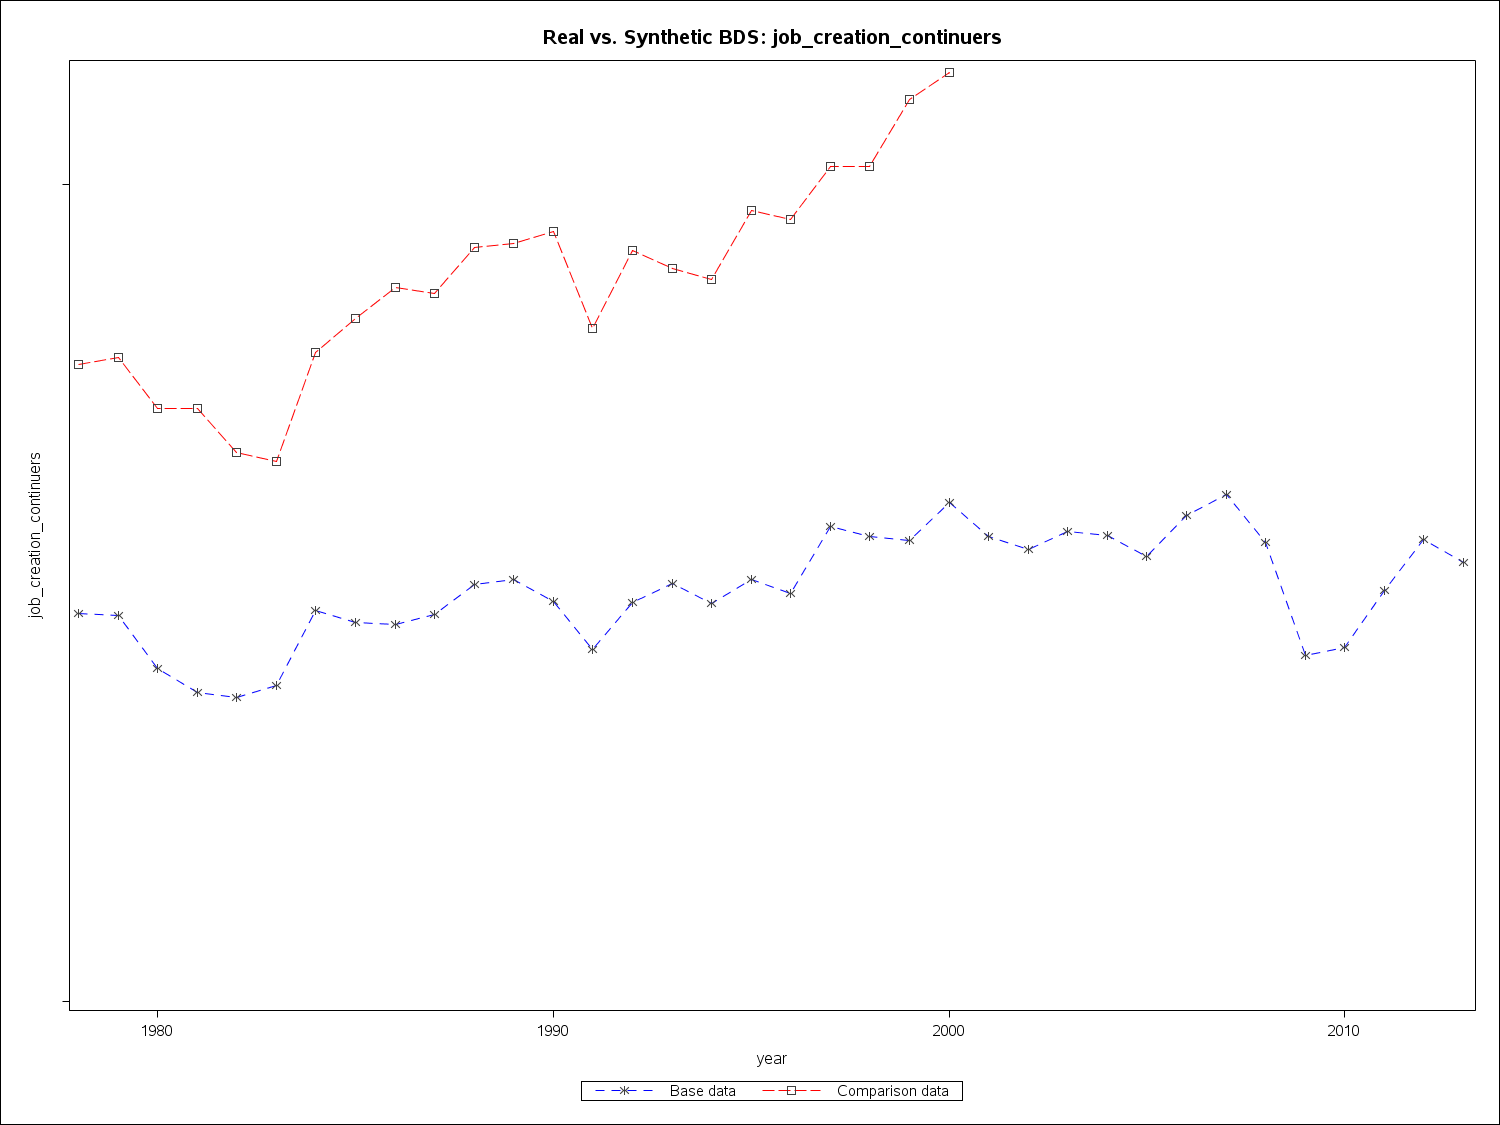
\includegraphics[width=0.45\textwidth]{results/graph_bds_real_vs_syn_job_creation_continuers}
%\end{figure}
%
%
%\begin{figure}
%\centering
%\caption{Differences between released and synthetic data\label{fig:pct_denom}\label{fig:pct_jc}}
%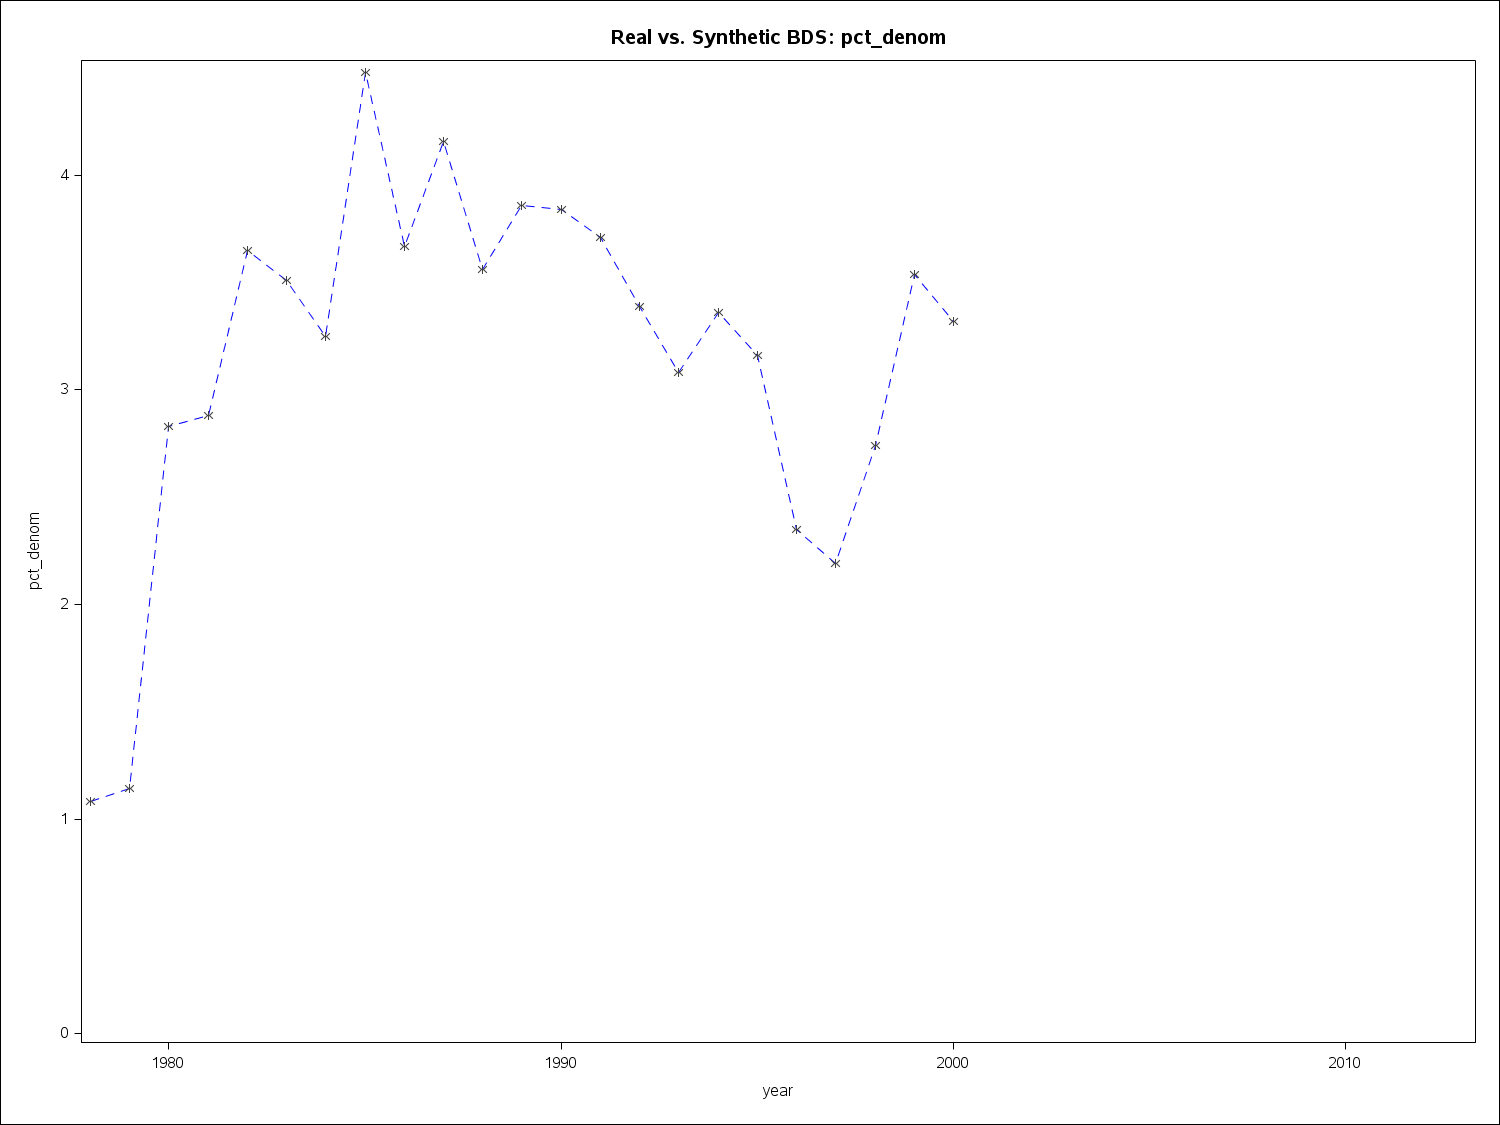
\includegraphics[width=0.45\textwidth]{results/graph_bds_real_vs_syn_pct_denom}
%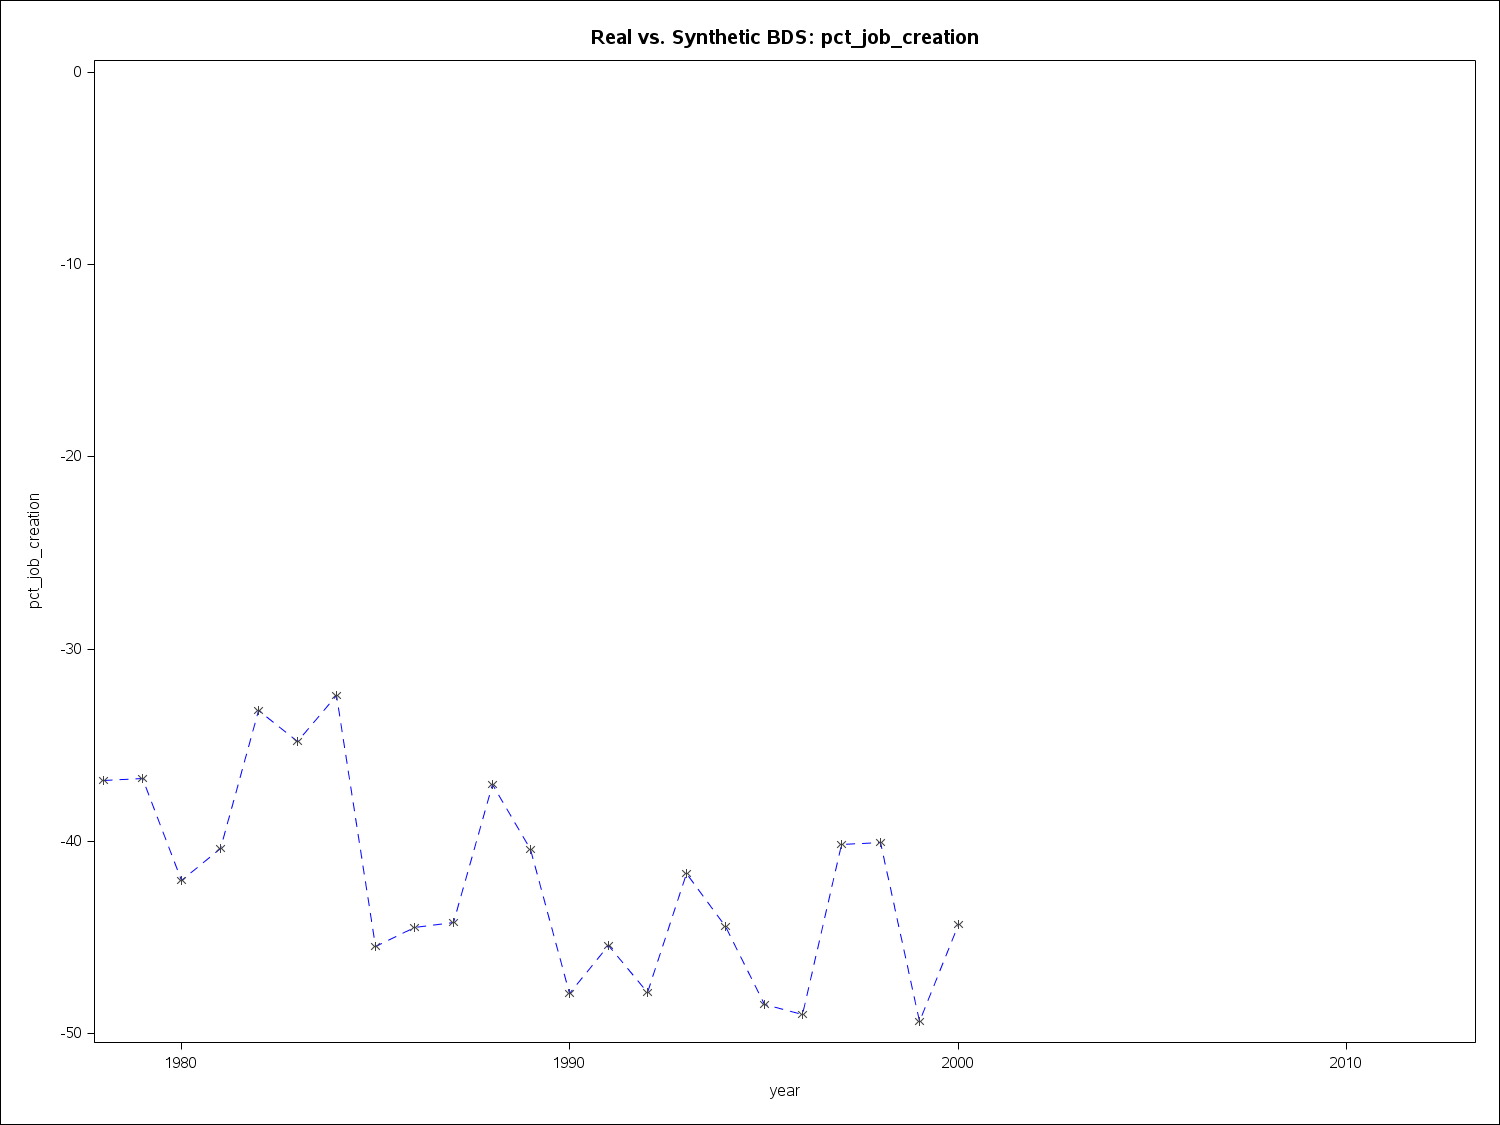
\includegraphics[width=0.45\textwidth]{results/graph_bds_real_vs_syn_pct_job_creation}
%
%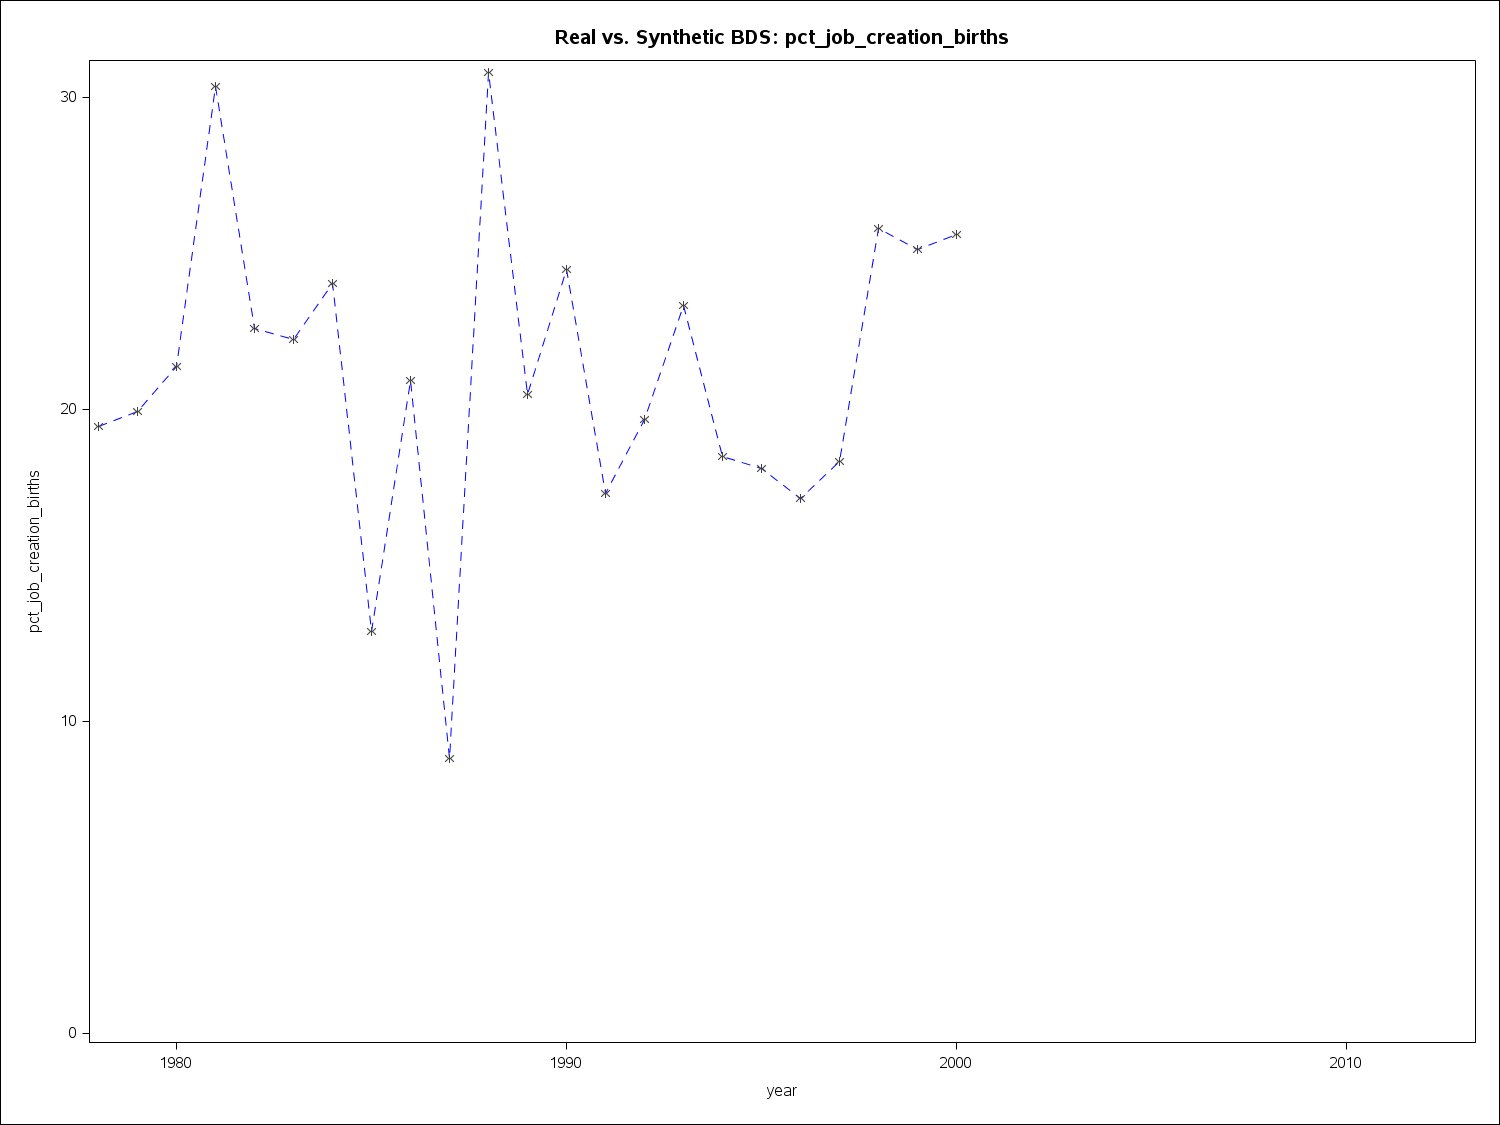
\includegraphics[width=0.45\textwidth]{results/graph_bds_real_vs_syn_pct_job_creation_births}
%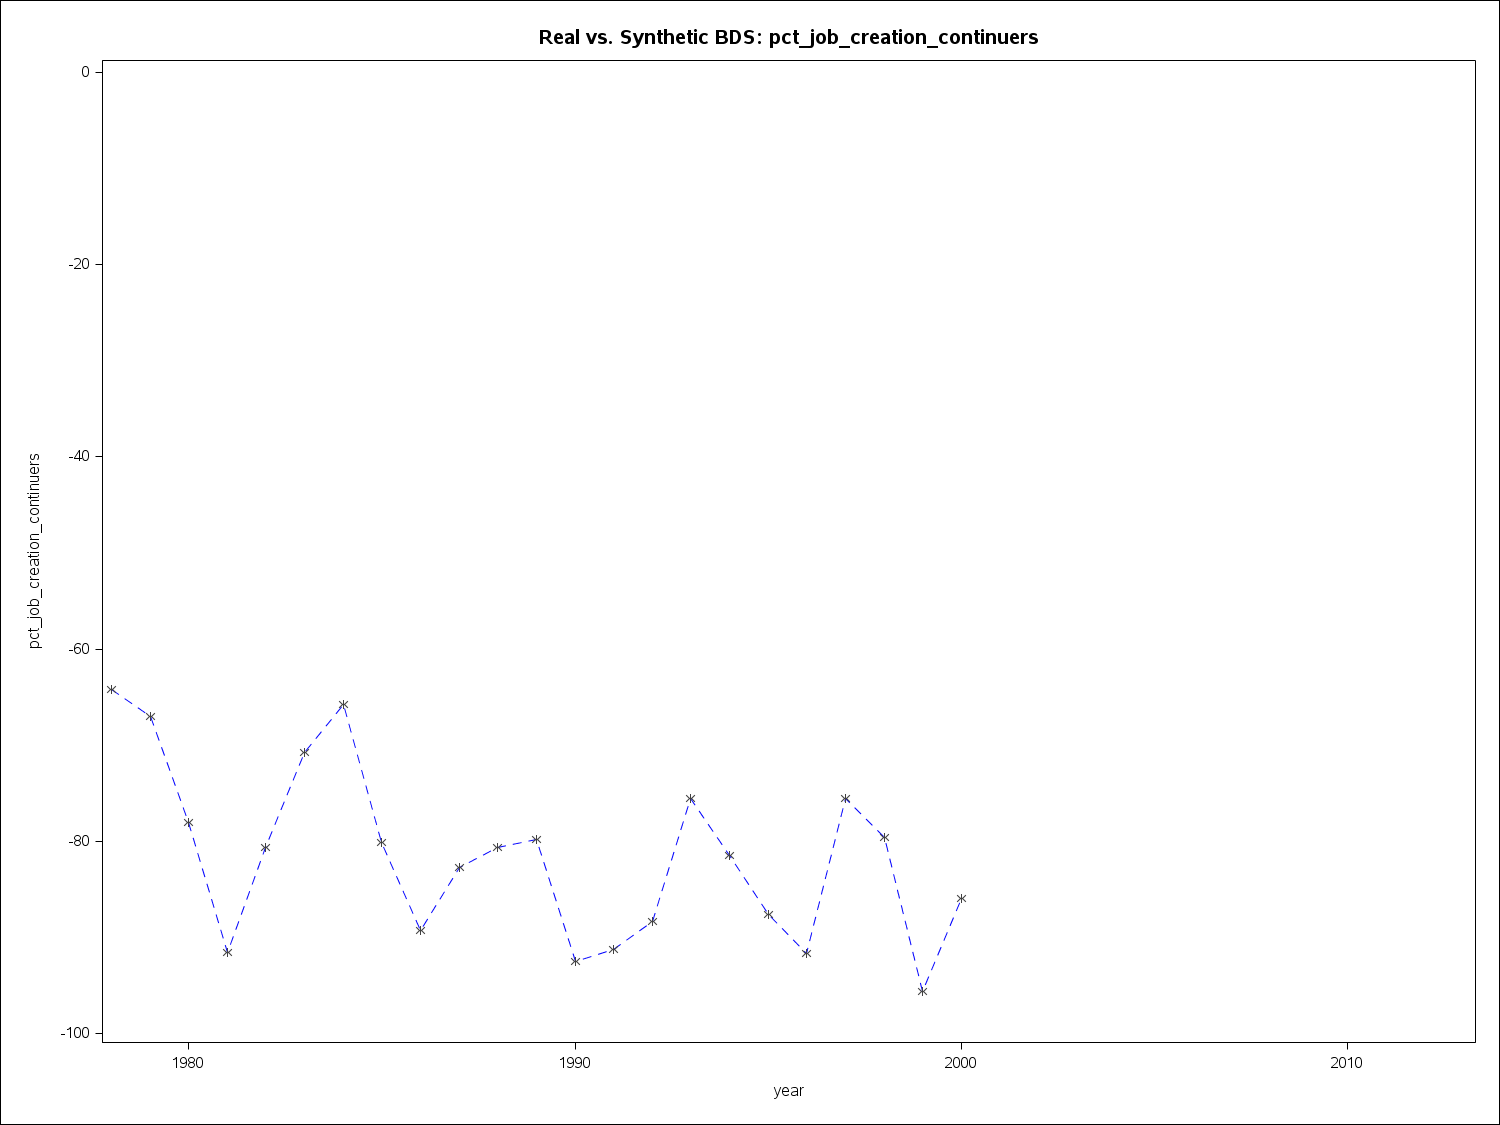
\includegraphics[width=0.45\textwidth]{results/graph_bds_real_vs_syn_pct_job_creation_continuers}
%\end{figure}


For comparison, there are no such differences at the most aggregated level between releasable and noise-infused tabulations (not shown). Percentage differences are less than two-tenths of a percent in all cases, as expected. 

%Section~\ref{sec:synthetic_method}, Table~TBD provides a 
%transition matrix for small values of the (confidential) $X_{k^\prime t}$ against $X_{k^\prime 
%t}^{s}$, $X_{k^\prime t}^{(i)}$, and 
%$X_{k^\prime t}^{(ii)}$, for several variables of interest (establishment births and deaths, job 
%creation and destruction, employment levels). (Table~TBD is being computed and/or pending 
%release at the time of submission of this document).

\subsection{Analytical validity}
%\margincomment{LARS}{We need to redo the histogram from Kinney et al (differences at the estab level) - can we (merge by LBDID)? Then need to do the same analysis, but at the cell level - histogram of differences in affected cells - those with suppressions/filled in, and the ancillary cells (t+1 through t+p) that are affected by the smoothing}
\label{sec:validity}
We turn to an assessment of analytical validity. In order to assess the analytical validity of each of 
the methods, we focus on simple 
%\margincomment{Lars}{cross-sectional distributional properties as well as }
time-series 
properties of  the $X_{k^\prime t}$. 
%\margincomment{Lars}{::For the cross-section, we compute for each year the Jenson-Shannon Divergence (JSD) metric for the entire table, and for those cells that ...:: HOW TO COMPUTE JSD when cells are missing?}
In particular, we 
estimate a AR(2) process for each of time-series generated by 
$X_{k^\prime t}$, $X_{k^\prime t}^{(0)}$, $X_{k^\prime t}^{(s)}$,  $X_{k^\prime t}^{(i)}$, $X_{k^\prime t}^{(ii)}$,   
$X_{k^\prime t}^{(iiw)}$, and $X_{k^\prime t}^{(iin)}$. 
We then assess, for each statistic $X$ under each of the regimes, the number of feasible regressions for $X_{k^\prime t}$ (for some values of $k$, data points may be missing because out-of-scope in certain time periods), and what fraction of the feasible regressions can be replicated under the alternate regimes. Table~\ref{tab:bds_e_pctmiss} presents these results for a number of variables.
%\margincomment{LV}{Table 3 would probably be better as a graph}
Conditional on a feasible estimation, we tabulate the fraction of $\rho_1$ estimates that are 
statistically significant at conventional levels (Table~\ref{tab:bds_e_pctmiss}).


%\begin{table}[p]
		\setlength{\tabcolsep}{6pt}
\caption{Analytic validity: Feasibility of AR(2) regressions \label{tab:bds_e_pctmiss}}
\centering
%\begin{tabular}{|lc|r|rrr|}\hline%
\csvreader[tabular=|l|r|r|rrr|rrr|r|,table head=\hline 
	&Number 
	&\multicolumn{8}{c|}{Percent} 
\\
Variable 
	&feasible 
	& \multicolumn{8}{c|}{Infeasible}                
\\
    & $X_{k^\prime t}$ 
    & $X_{k^\prime t}^{(s)}$ 
    & $X_{k^\prime t}^{(0)}$ 
    & $X_{k^\prime t}^{(i)}$
    & $X_{k^\prime t}^{(in)}$
    & $X_{k^\prime t}^{(ii)}$
    & $X_{k^\prime t}^{(iiw)}$
    & $X_{k^\prime t}^{(iin)}$
    & $X_{k^\prime t}^{(n)}$
    \\\hline,
	late after line=\\,late after last line=\\\hline]%
{results/r_e_agesz_all_missing.csv}{Variable=\V,number=\colz,missing1=\cola,missing2=\colb,missing3=\colc,missing4=\cold,missing5=\cole,missing6=\colf,missing7=\colg,missing8=\colh}%
{\V &  \colz & \cola & \colb & \colc & \cold & \cole & \colf & \colg &\colh}%
\end{table}

%\begin{table}[p]
	\setlength{\tabcolsep}{6pt}
\caption{Analytic validity: AR(2) regressions with significant parameters\label{tab:bds_e_pctsign}}
\centering
%\begin{tabular}{|lc|r|rrr|}\hline%
\csvreader[tabular=|l|rr|rrr|rrr|r|,table head=\hline 
	& \multicolumn{9}{c|}{Percent} 
\\
Variable 
	& \multicolumn{9}{c|}{significant}
\\
    & $\rho_{1}$ 
    & $\rho_{1}^{(s)}$ 
    & $\rho_{1}^{(0)}$ 
    & $\rho_{1}^{(i)}$
    & $\rho_{1}^{(in)}$
    & $\rho_{1}^{(ii)}$
    & $\rho_{1}^{(iiw)}$
    & $\rho_{1}^{(iin)}$
    & $\rho_{1}^{(n)}$
    \\\hline,
	late after line=\\,late after last line=\\\hline]%
{results/r_e_agesz_all_significant.csv}{Variable=\V,significantconf2=\colz,significant1=\cola,significant2=\colb,significant3=\colc,significant4=\cold,significant5=\cole,significant6=\colf,significant7=\colg,significant8=\colh}%
{\V &  \colz & \cola & \colb & \colc & \cold & \cole & \colf & \colg &\colh }%
\end{table}


Two measures of utility are also computed.
We compute \emph{coverage} as the 
percentage of regressions where the true $\rho_1$ lies within the confidence band around the 
coefficient estimated from the comparison $\rho_1^{*}$ for each of the tables generated by the 
different algorithms. Let $(L^{*},U^{*})$ be the 95\% confidence interval for $\rho_1^{*}$. 
\emph{Coverage} is the percentage of AR(2) estimates for which the ``true'' $\rho_1 \in  
(L^{*},U^{*})$. We 
generalize this measure  as suggested by \cite{tas2006}, and compute  the \emph{interval 
overlap measure} $J_k$. Consider the overlap of confidence intervals $(L,U)$ for $\rho_1$ (estimated from the confidential data) and $(L^{*},U^{*})$ for $\rho_1^*$. Let $L^{over} = \max (L,L^{*} )$ and $U^{over} = \min (U,U^{*})$. Then the average overlap in confidence intervals is

$$
J_k^{*} = \frac{1}{2} \left [ \frac{U^{over} - L^{over}}{U-L} + \frac{U^{over} - L^{over}}{U^*-L ^*}        \right ]
$$
We then average $J_k^{*}$ over all estimated AR(2) regressions.
Results are summarized in Tables~\ref{tab:bds_e_coverage} and \ref{tab:bds_e_jk}.

%\begin{table}[p]
		\setlength{\tabcolsep}{6pt}
\caption{Analytic validity: AR(2) regressions: 
Coverage\label{tab:bds_e_coverage}}
\centering
%\begin{tabular}{|lc|r|rrr|}\hline%
\csvreader[tabular=|l|r|rrr|rrr|r|,table head=\hline 
	& \multicolumn{8}{c|}{} 
\\
Variable 
	& \multicolumn{8}{c|}{Coverage}
\\
    & $\rho_{1}^{(s)}$ 
    & $\rho_{1}^{(0)}$ 
    & $\rho_{1}^{(i)}$
    & $\rho_{1}^{(in)}$
    & $\rho_{1}^{(ii)}$
    & $\rho_{1}^{(iiw)}$
    & $\rho_{1}^{(iin)}$
    & $\rho_{1}^{(n)}$
    \\\hline,
	late after line=\\,late after last line=\\\hline]%
{results/r_e_agesz_all_coverage.csv}{Variable=\V,coverage1=\cola,coverage2=\colb,coverage3=\colc,coverage4=\cold,coverage5=\cole,coverage6=\colf,coverage7=\colg,coverage8=\colh}%
{\V &  \cola & \colb & \colc & \cold & \cole  & \colf & \colg &\colh}%
\end{table}

%\begin{table}[p]
			\setlength{\tabcolsep}{6pt}
\caption{Analytic validity: AR(2) regressions: Interval 
overlap\label{tab:bds_e_jk}}
\centering
%\begin{tabular}{|lc|r|rrr|}\hline%
\csvreader[tabular=|l|r|rrr|rrr|r|,table head=\hline 
	& \multicolumn{8}{c|}{Interval} 
\\
Variable 
	& \multicolumn{8}{c|}{overlap}
\\
    & $J_k^{(s)}$ 
    & $J_k^{(0)}$ 
    & $J_k^{(i)}$
    & $J_k^{(in)}$
    & $J_k^{(ii)}$
    & $J_k^{(iiw)}$
    & $J_k^{(iin)}$
    & $J_k^{(n)}$
    \\\hline,
	late after line=\\,late after last line=\\\hline]%
{../results/r_e_agesz_all_Jk.csv}{Variable=\V,Jk1=\cola,Jk2=\colb,Jk3=\colc,Jk4=\cold,Jk5=\cole,Jk6=\colf,Jk7=\colg,Jk8=\colh}%
{\V &  \cola & \colb & \colc & \cold & \cole & \colf & \colg &\colh}%
\end{table}


%\margincomment{LV}{This whole section is new.}
We start by noting issues surrounding establishment births in both the synthetic and different 
releases of the observed data. Establishment births are particularly sensitive to identifier 
linkages, and regular improvements to the BDS microdata occur. On the other hand, it is one of 
the more difficult events to synthesize. This leads to discrepancies both between the synthetic 
and the confidential data, and between the public-use data released in September 2014 and the 
(preliminary) confidential tabulations from the June 2015 BDS microdata. 

We further note that the first two rows of each table serve as a control, reporting results for 
\textbf{emp} and 
\textbf{estabs}, never show any differences, since there are no observed suppressions. Job 
creation, which also is never suppressed, does show some differences in 
Table~\ref{tab:bds_e_jk} between \textbf{BDS$^{(0)}$} and \textbf{BDS$^{conf}$}, presumably 
due to data revisions.

Tables~\ref{tab:bds_e_coverage} and~\ref{tab:bds_e_jk} paint approximately the same picture. 
The synthetic data is sufficiently different to distort inferences in our application further away 
from the results obtained from the confidential data. While the published data, despite having 
suppressed cells, has an average $J_k$ of 92.6\%, filling in suppressions together with smoothing 
($n=4$) yields an average $J_k$ of 77.5\%. Clearly this is being driven by the increased use of 
statistically different synthetic data, since setting $n=0$ (and thus using less synthetic data in the 
tabulations) yields a higher average $J_k$. The results obtained through Algorithm~2 are 
qualitatively better, with very little variation across the parameter variations. Given the data 
vintage differences noted above, it is not reasonable to compare $J_k^{(0)}$ and $J_k^{(ii)}$ 
directly until consistent input data can be used.



